\chapter{Background}
\label{Background}

\begin{abstract}
This chapter introduces the theoretical and technical background required for the remainder of the thesis. It first presents the main concepts related to General Game Playing and imperfect-information games, including determinization and simulation-based search methods. It then introduces the two frameworks studied in this work, TAG and Ludii, with a particular focus on their approaches to hidden-information handling and game-state simulation.
\end{abstract}

%%% GGP %%%
\section{General Game Playing (GGP)}
GGP\cite{Genesereth2005GeneralGP} is a field of Artificial Intelligence that studies the design of agents capable of playing many different games through a common decision-making architecture. Unlike specialized game-playing systems, which are developed and optimized for a single game, GGP agents must operate without game-specific tuning. The rules of the game are provided as input, and the agent is expected to interpret them and generate strategies autonomously.

The field emerged prominently through the \hyperlink{http://ggp.stanford.edu/}{Stanford General Game Playing project}\footnote{Available at \url{http://ggp.stanford.edu/}} and the AAAI General Game Playing Competition, where games were described using the Game Description Language (GDL)\cite{Love+al:2006}. This approach introduced the idea of reusable game-independent AI agents capable of reasoning over arbitrary rule systems. Over the years, the competition contributed to the development of increasingly sophisticated GGP agents, including systems such as CADIAPLAYER\cite{finnsson2009cadiaplayer} and Woodstock, the latest champion of the General Game Playing competition\cite{koriche2017symmetry,koriche2017woodstock}.

Since then, GGP research has expanded toward increasingly diverse game domains, including video games through the General Video Game AI (GVGAI) framework\cite{Genesereth2005GeneralGP}, stochastic games, multi-player environment, and modern board games.

Modern tabletop games introduce several challenges that are uncommon in traditional perfect-information games such as Chess or Go. These games often include hidden information, stochastic events, large branching factors, and complex interactions between heterogeneous game components. As a result, agents can no longer rely solely on deterministic search over a fully observable game state. They must instead reason under uncertainty and evaluate actions using incomplete observations and hypothetical world states.

The General Game Playing community has long recognized this limitation. Extensions such as GDL-II were introduced to support imperfect-information and stochastic games within the GGP paradigm\cite{Genesereth2005GeneralGP}. These extensions allow game descriptions to represent hidden information and partial observability at the rule level. However, correctly handling imperfect information requires more than simply encoding hidden data in the game description. The simulation infrastructure itself must preserve uncertainty during search and prevent agents from accessing privileged information when generating hypothetical future states.

This distinction is central to the architectural differences between TAG and Ludii studied in this thesis. While both frameworks support hidden information at the game-definition level, they differ significantly in how uncertainty is preserved during simulation and state copying.

%%% (IM)PERFECT INFORMATIONS %%%
\section{Information}
\subsection{Perfect and Imperfect}
In game theory, a game is said to have perfect information if every player has complete knowledge of the game state at all times\cite{russell2020artificial}. Classical examples include Chess, Go, and Tic-Tac-Toe, where all pieces and previous actions are fully observable to every player throughout the game. In such environments, decision-making algorithms can reason directly over a single fully observable game state.
\begin{figure}[H]
    \centering % Centre l'ensemble des deux images sur la largeur de la page
    
    % Première image (gauche)
    \begin{minipage}[H]{0.45\textwidth}
        \centering
        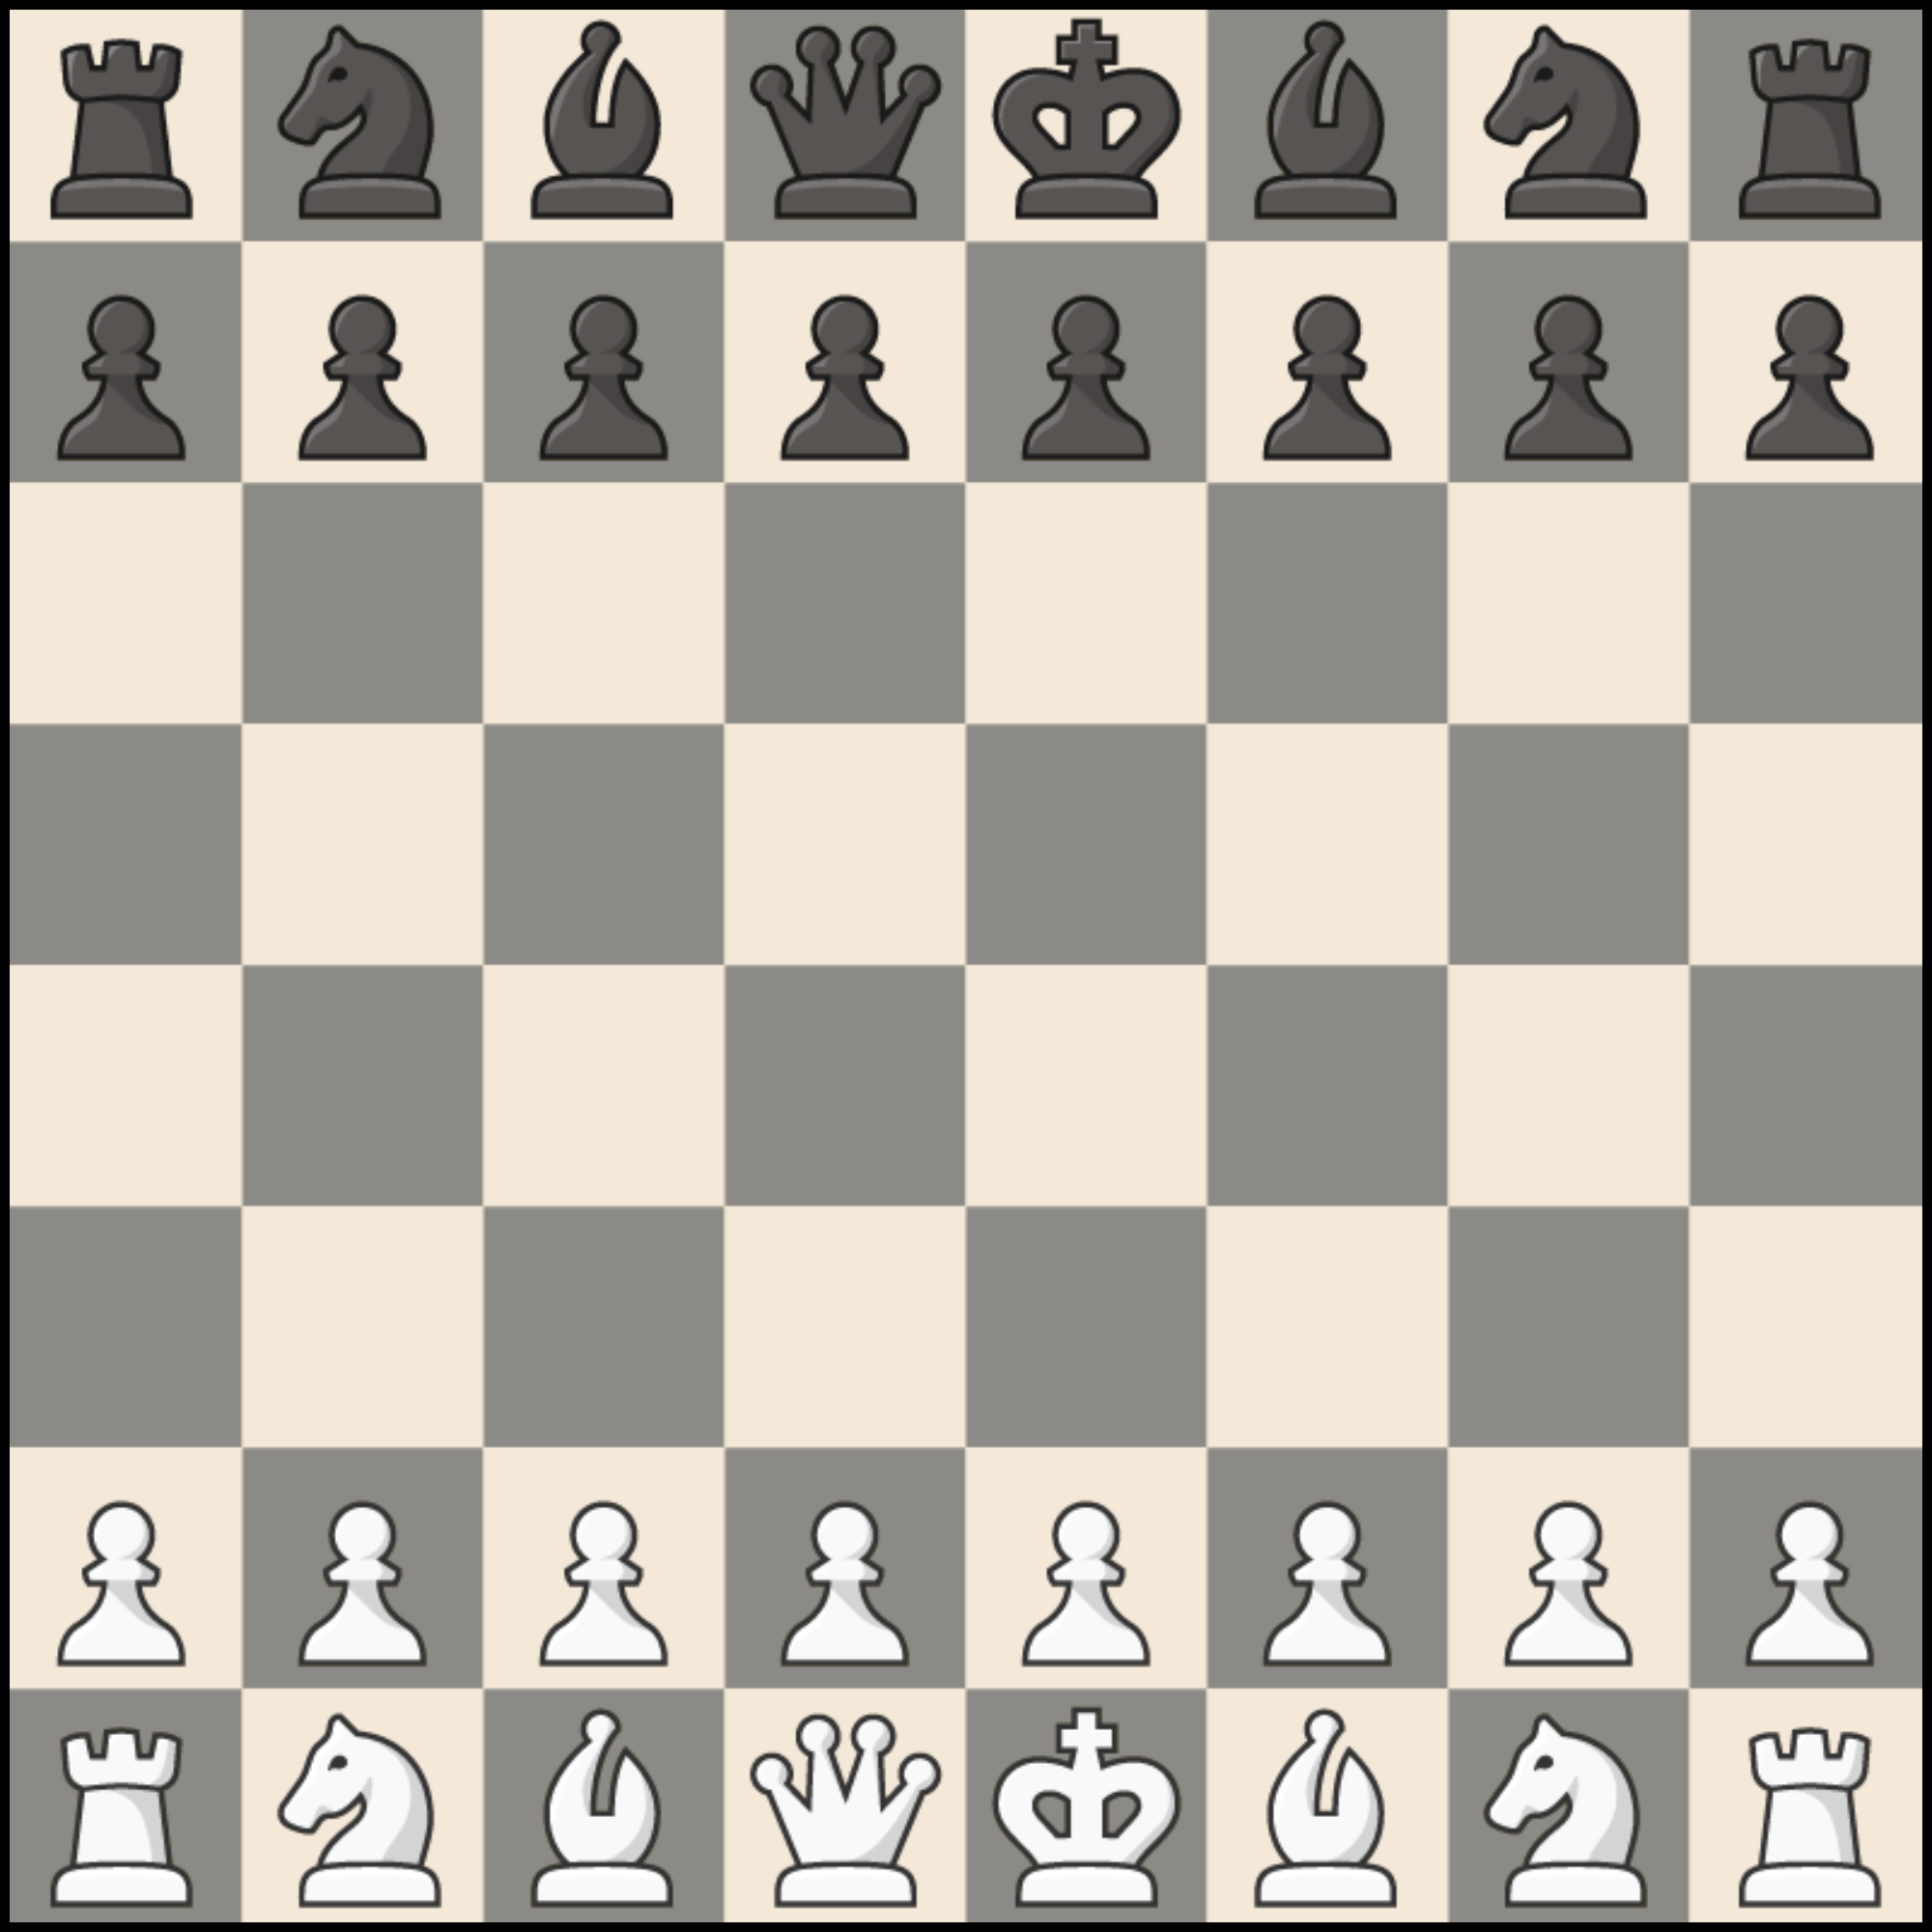
\includegraphics[width=0.75\textwidth]{figs/chess.png}
    \end{minipage}
    \hfill % Crée l'espace entre les deux images
    % Deuxième image (droite)
    \begin{minipage}[H]{0.45\textwidth}
        \centering
        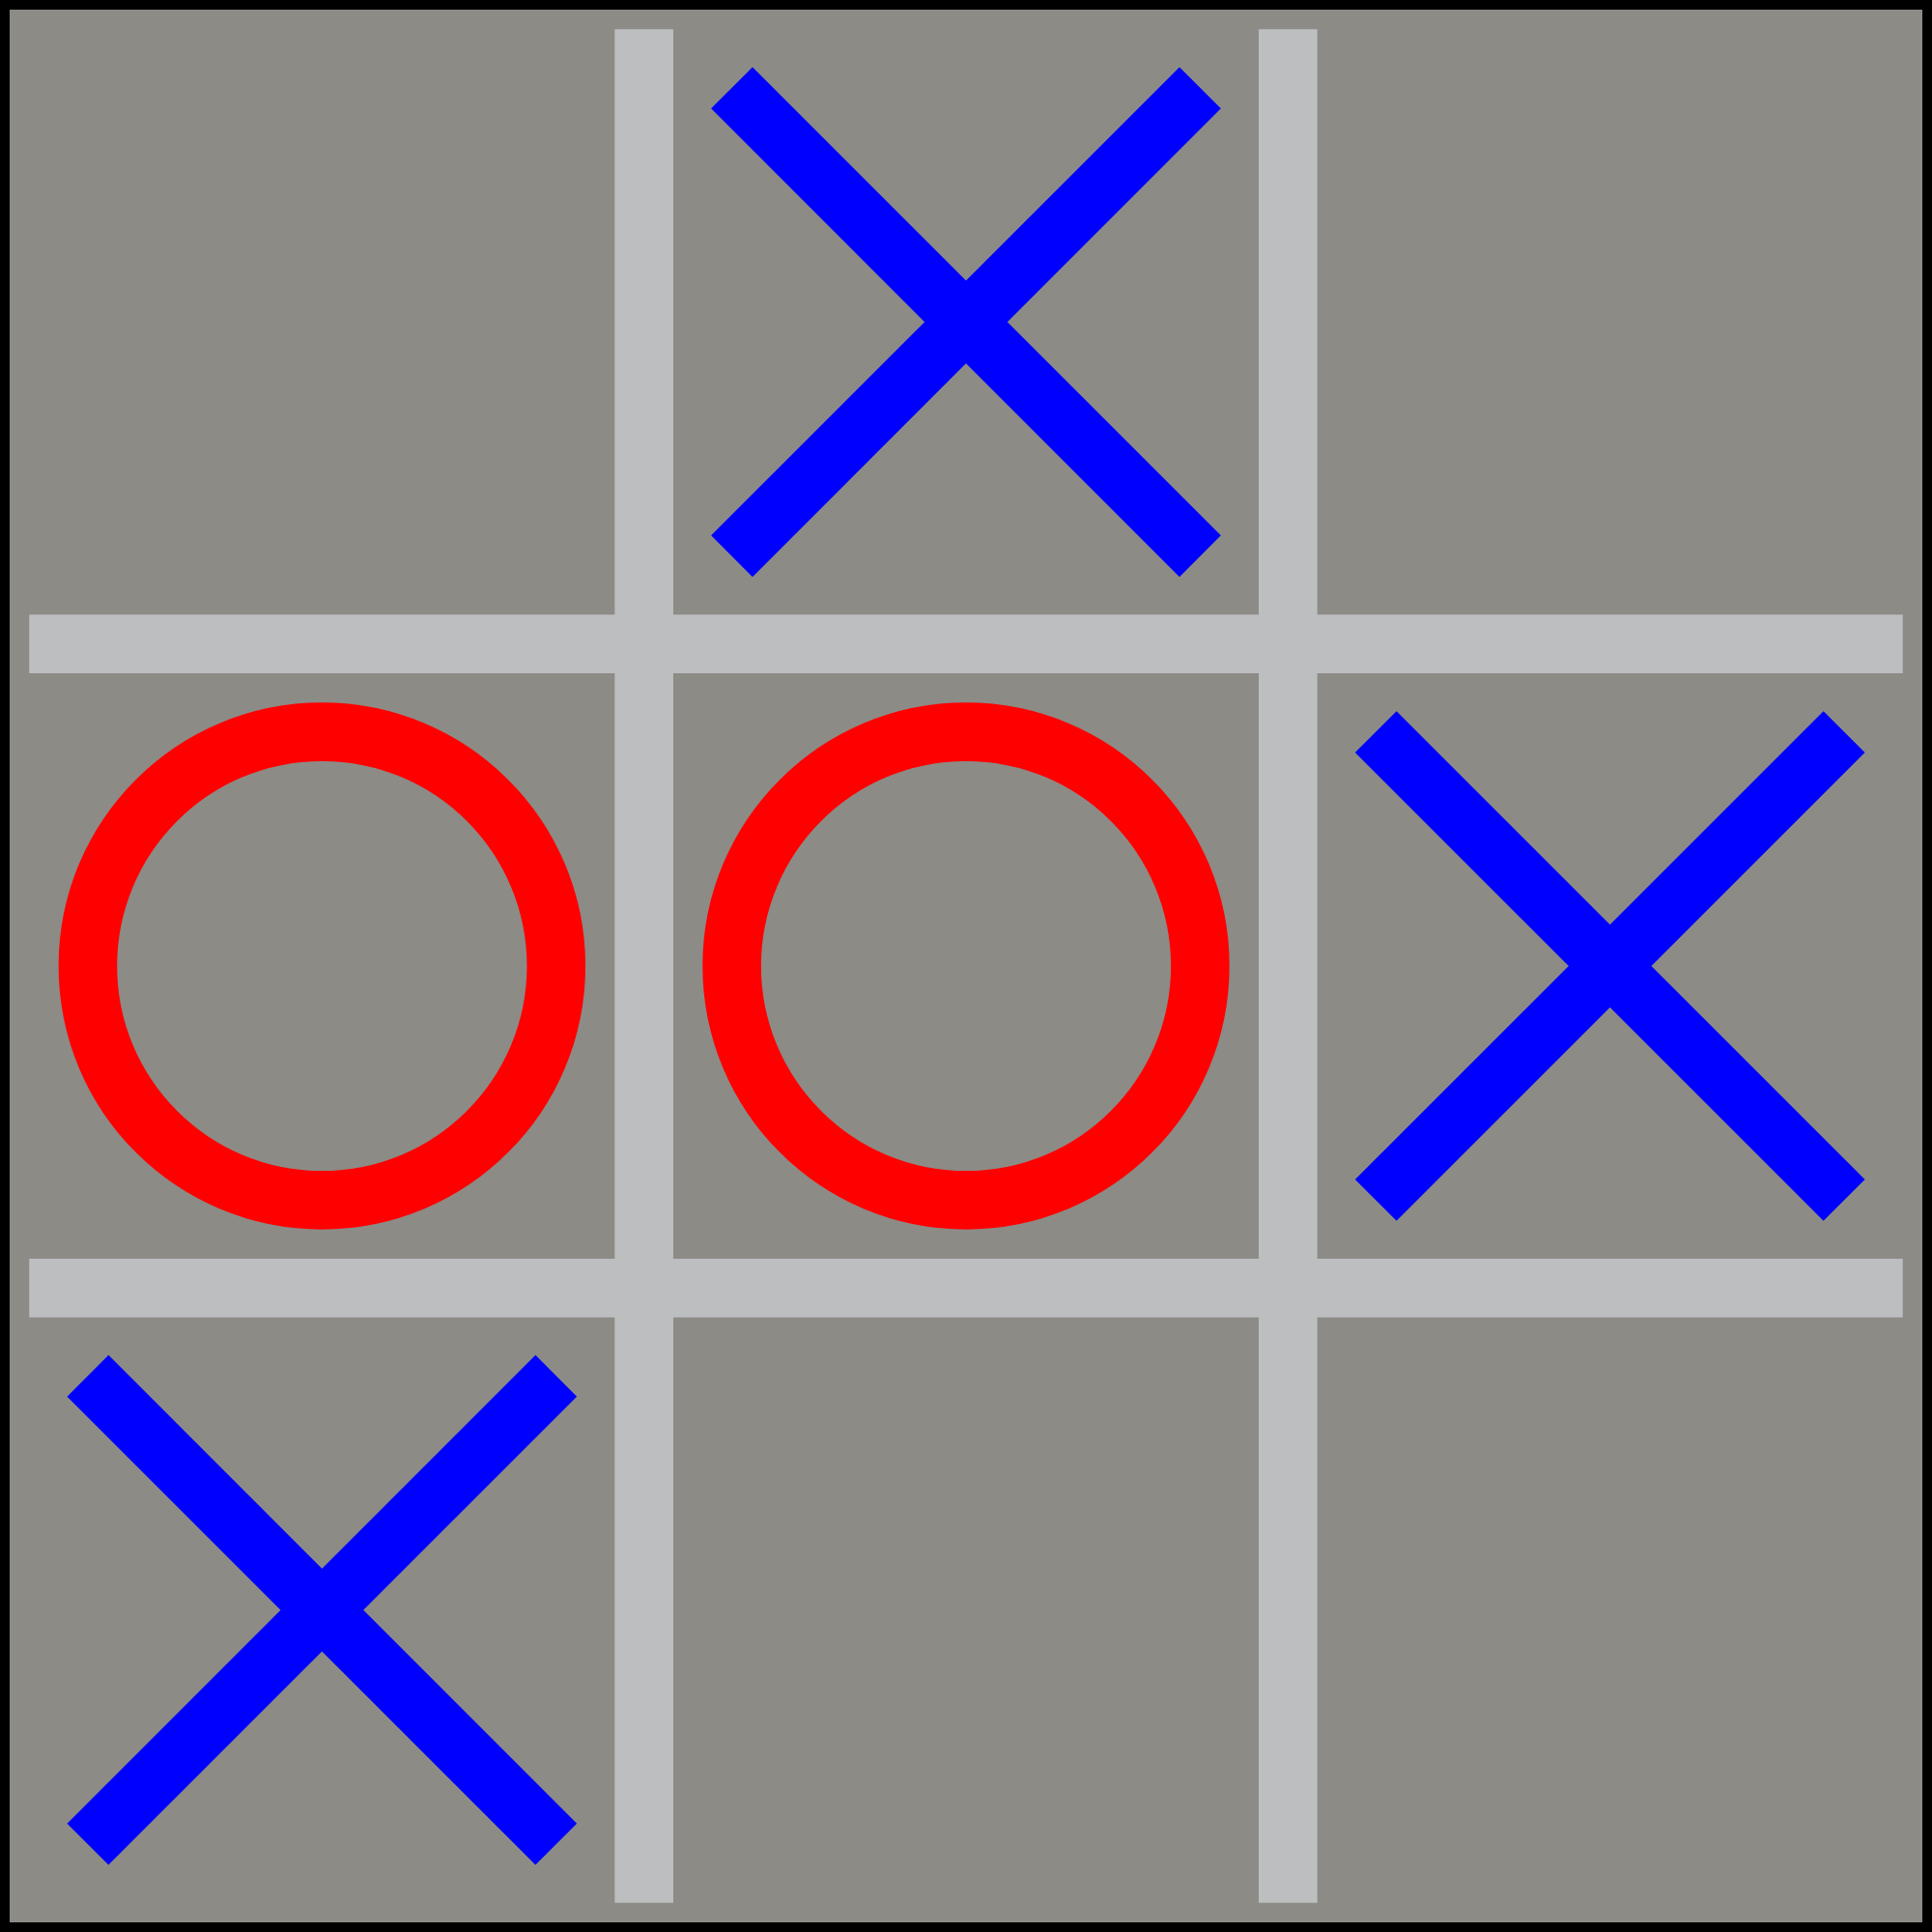
\includegraphics[width=0.75\textwidth]{figs/tictactoe.png}
    \end{minipage}

    \vspace{0.15cm} % Petit espace vertical avant la légende
    \captionsetup{justification=centering}
    \caption{In games like chess and TicTacToe, both players have a total visibility of the state of the game.}
    \label{fig:example_of_perfect_information_games}
\end{figure}

In contrast, a game has imperfect information when some aspects of the game state are hidden from at least one player\cite{russell2020artificial}. This hidden information may concern private cards, concealed pieces, secret objectives, or unknown positions on the board. Examples include Poker, Stratego, Battleship, and Mahjong. In these games, players must reason under uncertainty and make decisions based on incomplete observations. This distinction has major implications for Artificial Intelligence. In perfect-information games, agents can evaluate future actions by simulating deterministic transitions from a known state. In imperfect-information games, however, the agent must additionally reason about unknown elements of the environment and maintain hypotheses regarding the hidden parts of the game state.

\subsection{Different Types of Hidden information}
Hidden information can appear in many different forms depending on the game mechanics and the nature of the uncertainty involved\cite{kaelbling1998planning}. Previous work has explored several categories of imperfect-information structures, including hidden actions, hidden objectives, simultaneous decisions, stochastic uncertainty, and partially observable state transitions\cite{bowling2015heads}. The Valet game suite, for example, was specifically designed to study diverse forms of hidden information and uncertainty in tabletop games\cite{goadrich2026valet}. 

This thesis focuses on two forms of hidden state information that are particularly relevant for simulation-based reasoning in board games.

The first category concerns hidden identities. In this case, the location of a game object is visible, but its type or value is unknown. In Stratego, for example, players can observe the positions of opponent pieces without knowing their ranks. Similarly, in many card games, players know how many cards their opponents hold without knowing the exact cards themselves.

\vspace{0.5cm}
\noindent
\begin{minipage}[c]{0.45\textwidth}
    \centering
    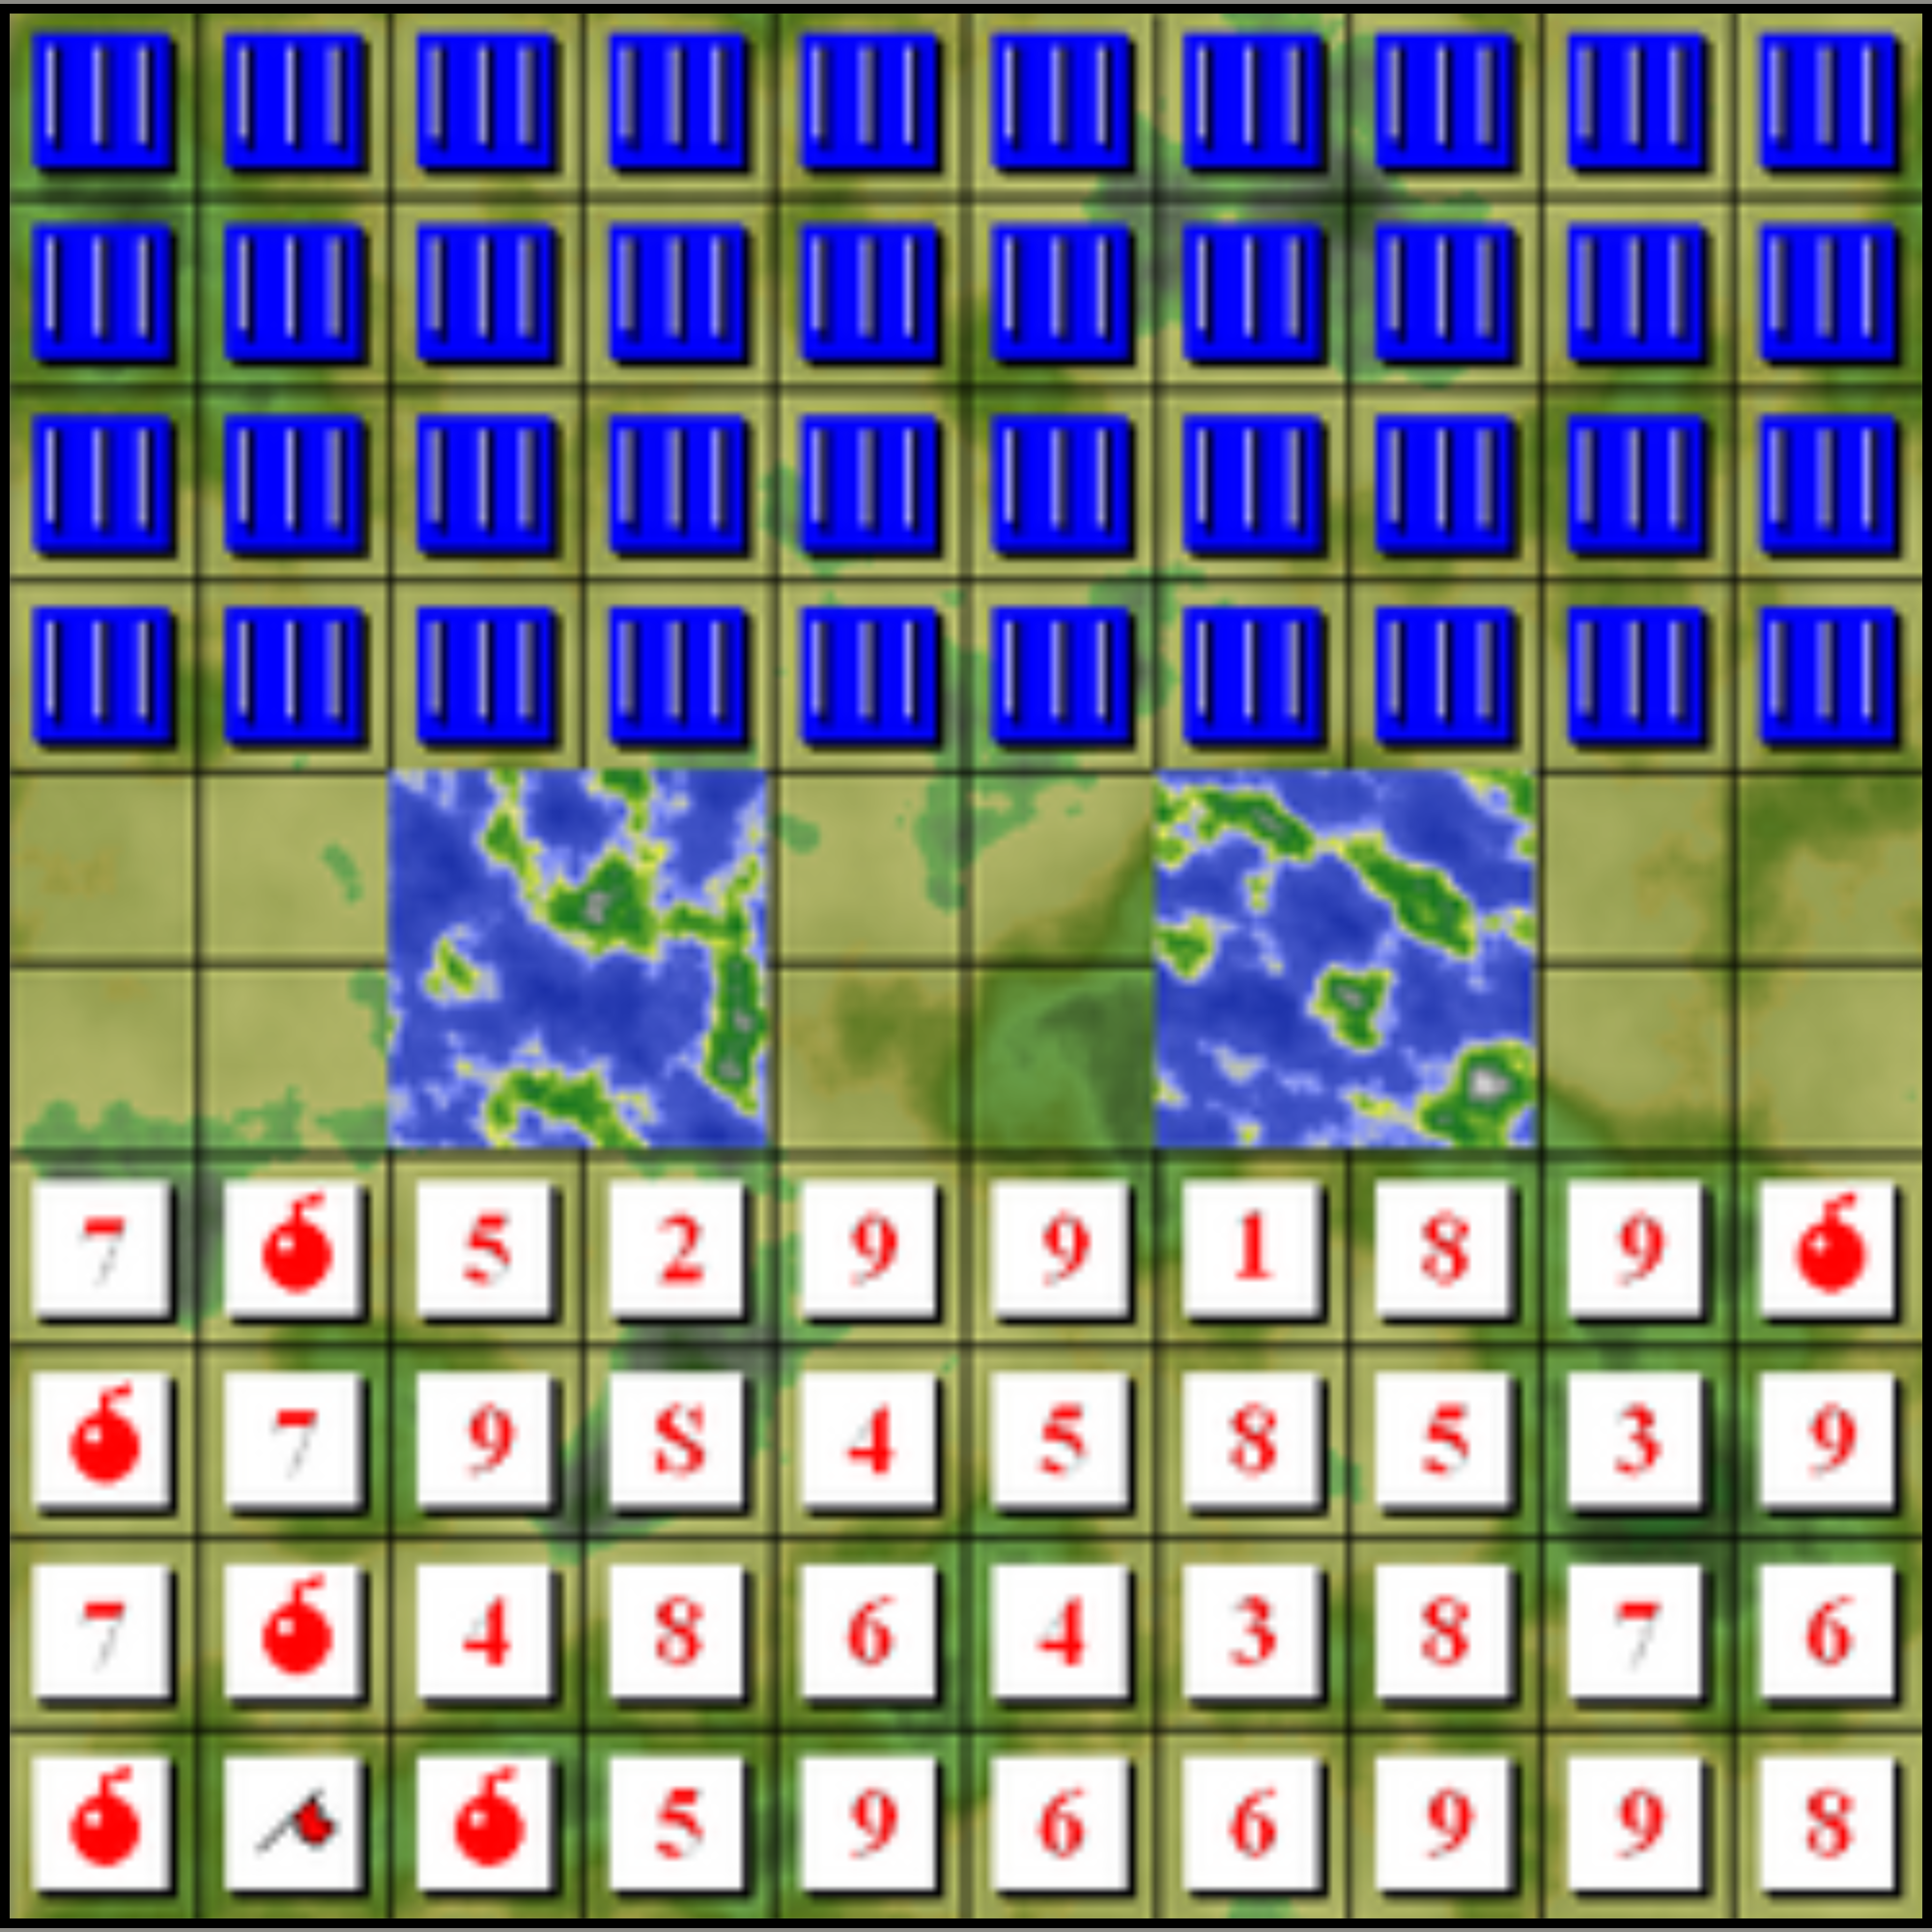
\includegraphics[width=0.80\textwidth]{figs/stratego.png}
    \captionsetup{hypcap=false}
    \captionof{figure}{We know the locations, but not the values.}
    \label{fig:stratego}
\end{minipage}
\hfill
\begin{minipage}[c]{0.50\textwidth}
    \textbf{Unknown identity of pieces}: The agent knows where a game object is, but not what it is. In Stratego, for instance, you can see that there is an opponent piece on a certain square, but you do not know its rank. In card games, you know your opponent has cards in hand, but not which ones.
\end{minipage}

The second category concerns hidden positions. In this case, the existence or location of objects is itself unknown. Battleship is a representative example: the opponent’s ships are completely hidden, and the player has no direct information regarding their positions on the grid.

\noindent
\begin{minipage}[H]{0.50\textwidth}
    \textbf{Unknown position of pieces}: The agent does not know where certain objects are at all. In Battleship, the opponent's ships are completely hidden: you do not even know in which region of the board they are. \textbf{This is the category that this thesis focuses on.}
\end{minipage}
\hfill
\begin{minipage}[H]{0.45\textwidth}
    \centering
    
\includegraphics[width=0.80\textwidth]{figs/battleship.png}
    \captionsetup{hypcap=false}
    \captionof{figure}{We don't know the locations of the enemy's ships and their values.}
    \label{fig:battleship}
\end{minipage}

This distinction has important consequences for AI reasoning. Hidden-identity games constrain uncertainty to known locations, whereas hidden-position games require the agent to reason over a significantly larger space of possible configurations. In hidden-position settings, the agent must first infer plausible locations before meaningful strategic planning can occur. Battleship belongs primarily to this second category and therefore provides a useful benchmark for studying determinization techniques under spatial uncertainty.

\subsection{Information Sets}
In extensive-form game theory, uncertainty is commonly represented through the notion of an Information Set\cite{Osborne1994}. In imperfect-information games, a player generally cannot determine the exact current game state because some elements of the environment remain hidden. Instead, multiple possible states may be consistent with the observations available to the player.

An Information Set therefore represents the collection of game states that are indistinguishable from the perspective of a given player at a particular moment in the game. Each state within the set is compatible with the player’s observations, the sequence of previously observed actions, and the known rules of the game. Two examples help illustrate this concept.

\textbf{In Poker}, if a card has been publicly revealed during gameplay, players may know part of an opponent’s hand while remaining uncertain about the remaining hidden cards. The corresponding Information Set contains all valid card distributions consistent with the revealed information.
\begin{figure}[H]
    \centering % Centre l'ensemble des deux images sur la largeur de la page

    % image
    \begin{minipage}[H]{\textwidth}
        \centering
        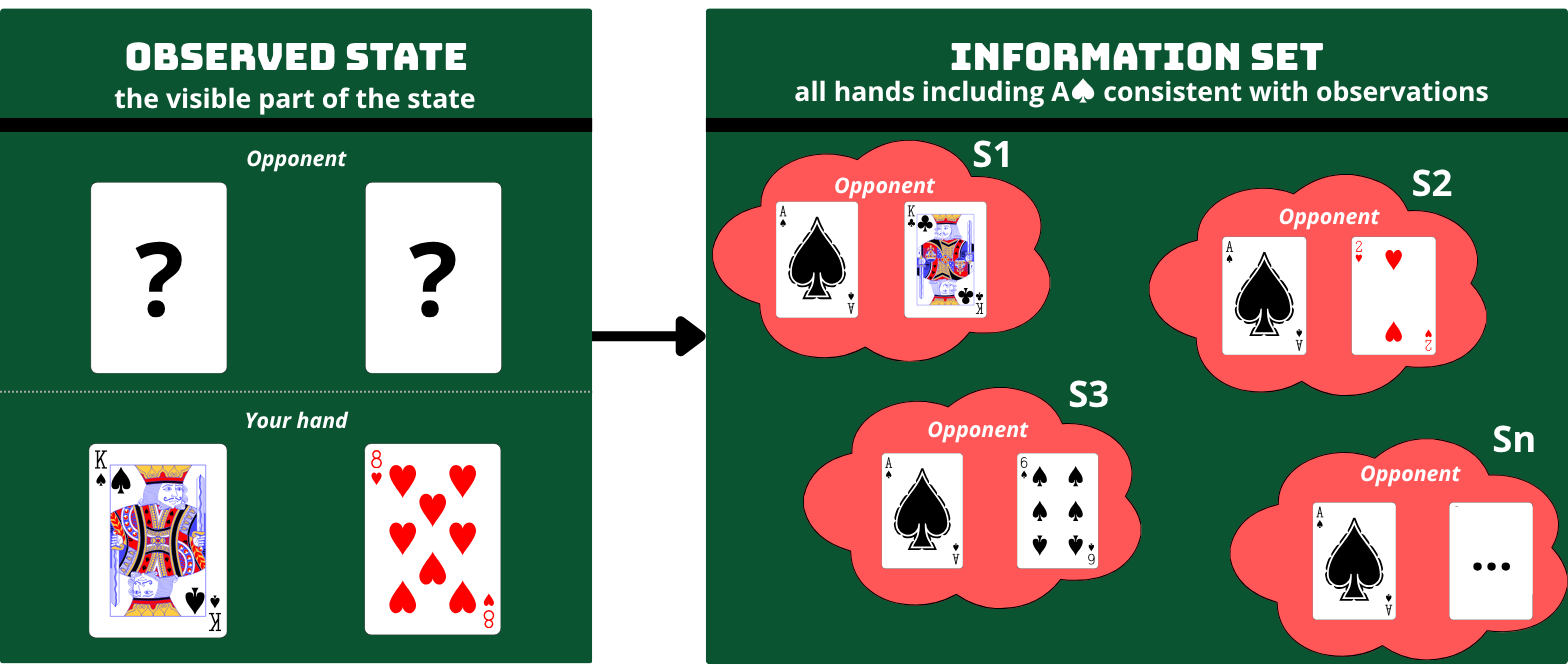
\includegraphics[width=1\textwidth]{figs/background/poker.png}
    \end{minipage}
    \captionsetup{justification=centering}
    \caption{All world configurations containing the Ace of Spades}
    \label{fig:poker}
\end{figure}

\textbf{In Battleship}, after observing a sequence of hits and misses, the Information Set contains all ship configurations compatible with these observations. Every additional shot progressively eliminates impossible configurations and reduces the number of plausible hidden states.

\newpage

Information Sets provide a formal framework for reasoning under uncertainty in imperfect-information games. However, explicitly representing all possible states quickly becomes computationally intractable in many practical settings. In Battleship, for example, the number of valid ship configurations at the beginning of the game is extremely large, making exhaustive enumeration impractical for simulation-based AI methods.

As a result, imperfect-information game AI systems often rely on approximate representations of uncertainty rather than explicit enumeration of complete Information Sets. This naturally leads to approaches based on belief states and determinization, which are introduced in the next section.

\subsection{Belief State and Determinization}
A common approach for reasoning under uncertainty consists in representing the player’s knowledge through a belief state: a probability distribution over all game states consistent with the observations available to the agent\cite{kaelbling1998planning}. As new observations become available during gameplay, this distribution can be updated to reflect changes in the player’s uncertainty regarding the hidden parts of the environment.

In theory, an optimal imperfect-information agent would reason directly over this belief distribution when selecting actions. In practice, however, maintaining and updating exact belief states is often computationally infeasible because the number of possible hidden configurations grows extremely rapidly in many games.

Consequently, practical imperfect-information AI systems frequently rely on approximate methods. One widely used approximation is determinization\cite{long2010understanding,cowling2012information}. Instead of reasoning over the full belief distribution, the agent samples or generates a plausible fully instantiated game state consistent with the currently available observations. The search algorithm then operates on this hypothetical state as if it were the true game state.

The quality of the determinization has a direct impact on the quality of the resulting simulations. If the generated hypothetical state is inconsistent with previous observations or highly implausible, the simulations performed by the agent may provide misleading evaluations and poor action recommendations.

Several simulation-based search algorithms rely on determinization techniques to operate in imperfect-information environments. These algorithms are introduced in the next section.

%%% AGENTS %%%
\section{Search Algorithms}
This section introduces the main simulation-based agents used throughout this thesis. These algorithms are representative baseline methods commonly used in GGP and modern board game AI research. While some were originally designed for perfect-information environments, several can be extended to imperfect-information settings through the use of determinization techniques.

\subsection{Random Agent}
The Random agent is the simplest possible baseline. At each turn, it selects one legal action uniformly at random without performing any evaluation or look-ahead.

Despite its simplicity, Random agents remain important in AI benchmarking because they provide a lower performance bound for comparison. Any search-based agent should consistently outperform a purely random policy in order to demonstrate meaningful strategic reasoning.

\subsection{One-Step Look-Ahead (OSLA)}
One-Step Look-Ahead (OSLA)\cite{gaina2020tag} is a greedy search method that evaluates the immediate consequence of each legal action before selecting a move. For every available action, the agent simulates a single forward step and evaluates the resulting state using a heuristic function, such as score estimation or game-specific features. The action producing the highest evaluation is then selected.

OSLA performs only shallow search and therefore cannot anticipate long-term consequences beyond the next state. Nevertheless, because it directly exploits information from simulated future states, it often provides significantly stronger performance than purely random play while remaining computationally inexpensive.

\subsection{Rolling Horizon Evolution (RMHC)}
Rolling Horizon Evolution (RHEA)\cite{perez2018rolling} is an online planning approach based on evolutionary optimization. Instead of constructing an explicit search tree, the agent maintains sequences of future actions representing candidate plans. These plans are iteratively modified through mutation operators and evaluated by simulating their execution in the game environment.

At each decision step, the best-performing action sequence is selected, the first action is executed, and the planning horizon is shifted forward for the next turn. Because the optimization process continuously replans during gameplay, the method is commonly referred to as a rolling horizon approach.

A simple and widely used variant is the Rolling Horizon Mutation Hill Climber (RMHC) \cite{perez2018rolling}, where candidate plans are optimized through repeated random mutations and greedy replacement. RHEA-based methods are particularly effective in environments with large action spaces where exhaustive tree search becomes difficult.

\subsection{Monte Carlo Tree Search (MCTS)}
Information Set Monte Carlo Tree Search (IS-MCTS)\cite{cowling2012information} extends MCTS to imperfect-information environments through the use of determinization. Instead of constructing the search tree from a single fully observable state, IS-MCTS repeatedly samples hypothetical game states consistent with the observations available to the player.

During search, simulations are therefore performed across multiple determinizations rather than a single known world state. This allows the agent to reason under uncertainty while still relying on standard forward simulations.

The effectiveness of IS-MCTS strongly depends on the quality of the determinization process. If sampled hypothetical states are inconsistent with previous observations or highly implausible, the resulting simulations may provide poor guidance for action selection. Consequently, the generation of coherent determinizations plays a central role in imperfect-information search performance.

\subsection{Move-Average Sampling Technique (MAST)}
The Move-Average Sampling Technique (MAST)\cite{chaslot2008progressive} is an enhancement commonly used with MCTS to improve rollout quality. Instead of selecting actions uniformly at random during simulations, MAST maintains statistics regarding the average reward historically associated with actions encountered across previous simulations.

These statistics are then used to bias rollout policies toward actions that performed well in the past, typically through epsilon-greedy or softmax selection strategies. By replacing purely random simulations with statistically informed rollouts, MAST can significantly improve search efficiency without requiring domain-specific heuristics.

Because MAST remains game-independent while improving simulation quality, it is frequently used as a general enhancement for GGP agents and modern board game AI systems.

%%% TBG VS MBG %%%
\section{Traditional Board Games \& Modern Board Games}
Traditional board games, such as Chess, Go, or Checkers, are typically characterized by \textbf{perfect information} and \textbf{simple, deterministic rules.} All players have full access to the complete game state at all times, and there is no hidden information. As a result, these games are well suited for classical AI techniques, including minimax search, alpha-beta pruning, and Monte Carlo Tree Search (MCTS)\cite{russell2020artificial}. Many early General Game Playing (GGP) systems were designed with this type of game in mind\cite{Genesereth2005GeneralGP}. On the other side, \textbf{modern board games} introduce a bigger variety of mechanics that significantly increase their complexity. These games often include \textbf{hidden information}, such as private hands of cards, secret objectives, or concealed board elements. They may also feature stochastic elements, large and dynamic action spaces, and complex interactions between game components. Examples include card-driven games, bluffing games, and games with fog-of-war or hidden spatial layouts. This difference has important consequences for AI research. While traditional board games allow agents to reason over a fully known and static game state, modern board games require agents to operate under \textbf{uncertainty.} The agent must make decisions based on incomplete observations and assumptions about unknown parts of the game state. As a result, AI techniques designed for perfect-information games often perform poorly or become invalid when applied directly to modern board games. Therefore, supporting modern board games requires frameworks that can explicitly represent hidden information and provide mechanisms for reasoning under uncertainty. This distinction motivates the need for platforms such as TAG and highlights the limitations of existing GGP systems that were originally designed for traditional games.

%%% TAG %%%
\section{The Tabletop Games Framework (TAG)}
\subsection{Overview of TAG}
TAG\cite{gaina2020tag} is a Java-based research framework designed for benchmarking AI agents on modern tabletop games. The framework was developed to address limitations of earlier GGP systems, which primarily focused on classical perfect-information games. TAG instead targets modern tabletop environments that frequently involve stochasticity, multi-player interactions, and hidden information.

TAG currently includes implementations of numerous modern board and card games, together with a standardized experimental infrastructure for AI evaluation\cite{gaina2023design}. The framework provides reusable implementations of several simulation-based agents, tournament management tools, and detailed logging systems capable of recording gameplay statistics such as branching factors, action-space sizes, hidden-information levels, and win rates. This infrastructure facilitates controlled and reproducible experimentation across multiple games and agent configurations.

Beyond academic research, the framework has also contributed to practical applications in tabletop game development. In particular, TAG served as the foundation for \hyperlink{https://www.tabletoprnd.co.uk/}{Tabletop R\&D}\footnote{Available at \url{https://www.tabletoprnd.co.uk/}}, a spin-out initiative focused on AI-assisted board game analysis, balancing, and automated playtesting. This illustrates the growing practical relevance of modern tabletop game AI beyond purely academic benchmarking.

\subsection{Code-First Design}
TAG follows a code-first design philosophy in which games are implemented directly in Java rather than described through a dedicated game description language. This approach provides developers with substantial flexibility regarding game logic, state representation, and simulation behavior.

Because games are implemented programmatically, developers can directly control hidden-information handling, optimization strategies, and custom mechanics that may be difficult to express declaratively. This flexibility is particularly important for imperfect-information research, where the way game states are copied and observed during simulations has a direct impact on agent behavior.

The main limitation of this approach is scalability. Implementing a new game requires writing a dedicated Java implementation, which demands significantly more development effort than declarative game-description systems such as Ludii.

\subsection{Architecture}
\textbf{TAG} uses an \textbf{MVC (Model-View-Controller)} architecture, which is a standard software design pattern that separates data (\textbf{M}odel), visual presentation (\textbf{V}iew), and decision logic (\textbf{C}ontroller). 
In the context of game AI, this makes it easy to implement new games and plug in new AI agents without modifying the core framework.



The \textbf{M}odel consists of three abstract classes that must be implemented for each game:
\begin{itemize}
    \item The \textbf{AbstractGameState} stores everything about the current game state: the board, the pieces, the scores, the current player, and any hidden information.

    \item The \textbf{AbstractForwardModel} handles the game logic. It generates the list of legal actions via \textsc{\_computeAvailableActions()}, applies them to the game state, and checks end conditions in \textsc{\_afterAction()}.

    \item The \textbf{AbstractParameters} stores the configurable parameters of the game, such as grid size or ship sizes in Battleship for example.
\end{itemize}
Implementing a new game in TAG requires writing these three classes. The framework handles everything else (turn management, logging, tournament running, and result analysis).

\medskip

The \textbf{V}iew consists of GUI components: \textbf{AbstractGUIManager} and \textbf{\textit{game-specific board views}} that render the game state visually. The GUI is optional and not required for AI experiments. 

\medskip

The \textbf{C}ontroller is \textbf{Game.java}, which orchestrates the game loop. At each turn, it calls the forward model to compute available actions, passes them to the current agent, and applies the chosen action to the game state.

\begin{figure}[H]
    \centering % Centre l'ensemble des deux images sur la largeur de la page
    
    \begin{minipage}[H]{1\textwidth}
        \centering
        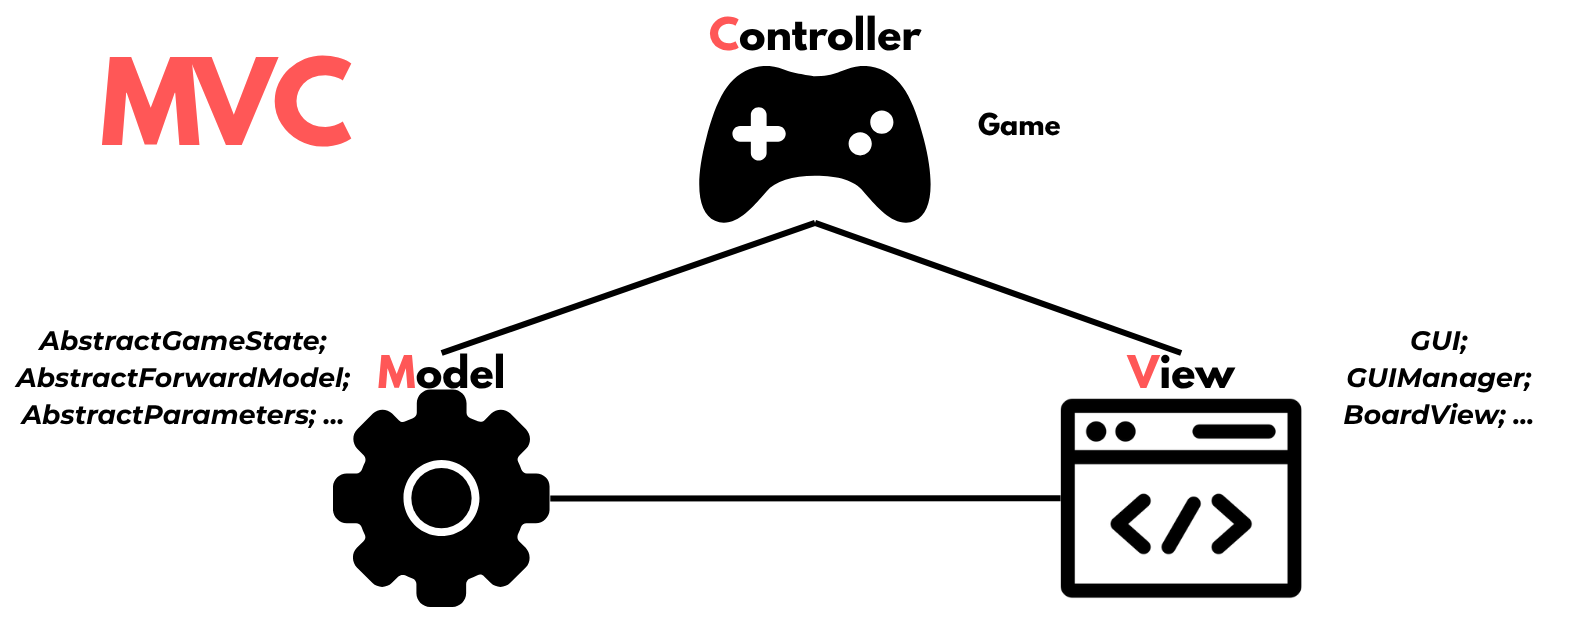
\includegraphics[width=1\textwidth]{figs/background/MVC.png}
    \end{minipage}

    \vspace{0.15cm} % Petit espace vertical avant la légende
    \captionsetup{justification=centering}
    \caption{TAG's Model-View-Controller (MVC) Architecture}
    \label{fig:TAG_MVC_Architecture}
\end{figure}

\subsection{Agent Interface and State Copying}
AI agents in TAG extend the AbstractPlayer class and implement a decision function that selects an action from the current game state and the list of legal actions.

\begingroup
\captionsetup[lstlisting]{justification=centering}
\begin{lstlisting}[language=Java, caption={Abstract method for selecting an action from available legal moves}, label=lst:basic-deter, basicstyle=\ttfamily\small, columns=fullflexible, keepspaces=true]
public abstract AbstractAction _getAction(AbstractGameState gameState, List<AbstractAction> possibleActions);
\end{lstlisting}
\endgroup

A key architectural feature of TAG is its support for player-specific state copies. During simulations, agents do not necessarily receive the true underlying game state. Instead, the framework allows the game implementation to generate customized observations through player-dependent copy mechanisms.

This design is particularly important for imperfect-information games. Hidden information can be masked, randomized, or replaced with coherent hypothetical states before simulations are performed. As a result, agents reason over observations and determinizations that are consistent with the information available to the corresponding player rather than over privileged hidden information.

This explicit control over simulation copies makes TAG especially suitable for research on imperfect-information reasoning and determinization techniques.

\subsection{Current Limitations}
Despite its flexibility for AI experimentation, TAG also presents several limitations. Its game library remains relatively small compared to large-scale General Game Playing systems such as Ludii, and every new game requires a dedicated manual implementation in Java.

Furthermore, because TAG does not rely on a declarative game description language, rapidly prototyping or modifying game variants can require substantial development effort. These limitations motivate the interest in complementary frameworks capable of supporting much larger game libraries while still enabling robust imperfect-information reasoning.


%%% LUDII %%%
\section{The Ludii General Game Playing System}
\subsection{Overview of Ludii}
Ludii\cite{piette2020ludii} is a General Game Playing framework designed to support a very large and diverse collection of games through a unified game description system\cite{piette2020ludii}. Unlike code-first frameworks such as TAG, Ludii follows a data-first approach in which games are described declaratively using a dedicated language known as the Ludii Game Description Language (.lud)\cite{browne2020ludii_language}. The framework originated from the Digital Ludeme Project\cite{browne2022dlpworkshop}, an initiative focused on the historical reconstruction, analysis, and study of traditional games through computational methods. Ludii was developed as the central software platform supporting this effort by providing a unified representation system capable of modeling games from many different historical periods and cultural traditions\cite{crist2024ludii_database}. Today, the framework continues to be actively maintained and is used extensively within the GameTable COST Action research network\cite{piette2024gametable_kickoff} for experimentation, game analysis, and AI benchmarking across large collections of tabletop games\cite{browne2023ludii}.

Ludii was originally designed around the concept of ludemes, which represent conceptual units of game rules and mechanics\cite{piette2021concepts}. By combining ludemes hierarchically, the framework can represent a wide range of board, card, dice, and multiplayer games within a common formal system. Ludii currently includes \hyperlink{https://ludii.games/library.php}{more than one thousand playable games from diverse cultural and historical contexts}\footnote{Available at \url{https://ludii.games/library.php}}.

One of Ludii’s major strengths is its scalability for GGP research. Because games are described declaratively rather than implemented manually in code, new games and variants can often be created rapidly with relatively limited development effort. This makes Ludii particularly attractive for large-scale experimentation, comparative game studies\cite{rautureau2026gametable_opening}, procedural game generation\cite{todd2024gavel}, and automated AI benchmarking across diverse game libraries\cite{piette2019ludii_rbg}.

In addition to classical perfect-information games such as Chess and Go, Ludii also supports stochastic and imperfect-information games through dedicated language constructs. Hidden information can be specified declaratively within the game description, allowing the framework to represent mechanisms such as hidden hands, concealed identities, and partially observable game elements.

However, representing hidden information at the game-description level does not necessarily guarantee correct imperfect-information reasoning during simulation. As discussed in the following sections, the way game states are copied and exposed to agents during search plays a critical role in determining whether uncertainty is properly preserved during AI simulations.

\subsection{Data-First Design}
Unlike code-first frameworks such as TAG, Ludii represents games through declarative `.lud` descriptions composed of ludemes. Rather than implementing game logic manually in procedural code, developers define games through hierarchical combinations of reusable rule components.

This design introduces an additional abstraction layer between the game definition and the underlying simulation engine. AI agents therefore interact with generic game representations generated from the declarative description rather than with manually customized game implementations.
For instance, the following extract from \textbf{Battleships.lud} describes how hidden information is set up at the start of the game:
\begin{center}
    \begin{verbatim}
        (set Hidden (sites P1 "Defence") to:P2)
        (set Hidden (sites P2 "Defence") to:P1)
    \end{verbatim}
\end{center}
This tells Ludii that player 1's defence zone is hidden from player 2, and vice versa. The hidden information is encoded directly in the game description, no Java code is needed.

Such abstraction provides important advantages for GGP research. Because games share a common internal representation structure, the same AI agents, analysis tools, and experimental pipelines can be reused across many different games with limited adaptation.

However, this abstraction also creates challenges for imperfect-information reasoning. In code-first systems, developers can explicitly customize how hidden information is exposed to players during simulations. In declarative systems such as Ludii, hidden-information handling must instead emerge from generic engine-level mechanisms capable of operating across many different game types.

As a consequence, correctly preserving uncertainty during simulation becomes an architectural problem extending beyond the game description itself. This distinction is central to the hidden-information limitations studied in this thesis.

\subsection{Architecture}
Ludii transforms declarative .lud descriptions into executable game representations through an internal compilation process. Once compiled, games are executed through a collection of generic runtime objects responsible for storing game states, applying rules, and managing simulations.

\begin{figure}[H]
    \centering % Centre l'ensemble des deux images sur la largeur de la page
    
    \begin{minipage}[H]{1\textwidth}
        \centering
        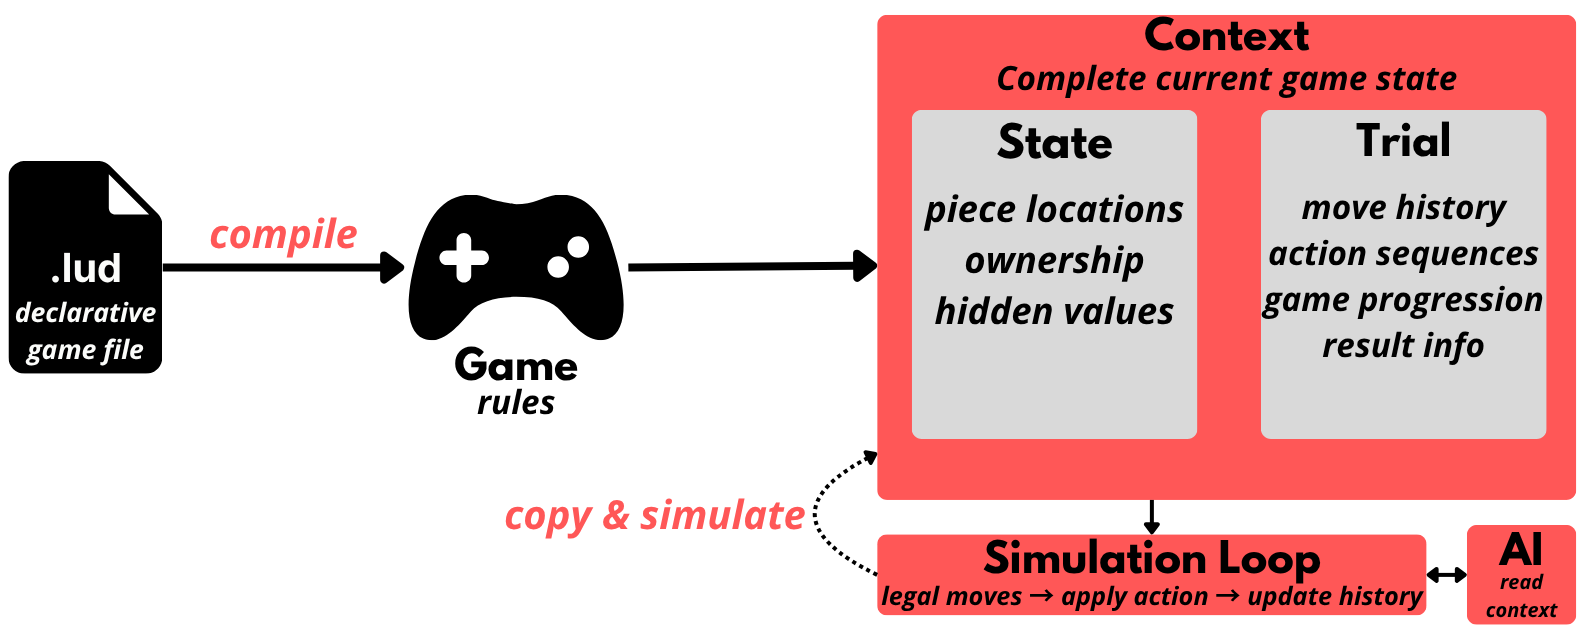
\includegraphics[width=1\textwidth]{figs/background/ludiiARCH.png}
    \end{minipage}

    \vspace{0.15cm} % Petit espace vertical avant la légende
    \captionsetup{justification=centering}
    \caption{Ludii's Architecture}
    \label{fig:ludii_architecture}
\end{figure}

One of the central runtime objects is the Context, which represents the complete current state of an ongoing game. The Context contains all information required to continue gameplay, including board configurations, player data, hidden information, scores, random generators, and references to previous actions. The Context itself contains two important substructures:
\begin{itemize}
    \item \textbf{State}, which stores the current mutable state of the game, such as piece locations, ownership, hidden values, and phase information.

    \item \textbf{Trial}, which records the history of actions performed during the game, including move sequences and game progression information.
\end{itemize}
Together, these structures provide the information required by AI agents during gameplay and search. Game progression is managed through generic rule execution mechanisms. At each decision step, Ludii generates the legal moves available from the current Context, applies selected actions to produce successor states, and updates the corresponding game history. Because this process is implemented generically at the engine level, the same simulation infrastructure can operate across many different game types without requiring game-specific AI implementations. Simulation-based agents typically evaluate future actions by repeatedly copying the current Context and performing forward simulations on the copied state. This mechanism is efficient for perfect-information games because the copied context fully represents the exact current game state.

However, in imperfect-information environments, the copied Context may also contain hidden information that should not be accessible to the acting player during search. Consequently, the semantics of state copying become particularly important for preserving uncertainty correctly during simulations. This issue is examined in the following sections.

\subsection{Hidden Information Representation}
Ludii supports imperfect-information games through dedicated language constructs integrated directly into the .lud description system. These constructs allow game designers to specify which parts of the game state are visible or hidden to different players during gameplay.

Hidden information in Ludii is represented primarily through visibility rules associated with game elements and state variables. Depending on the game, these rules may hide the identity of pieces, their positions, the ownership of components, private hands, or other game-specific information from selected players.

The framework distinguishes several forms of hidden information, including hidden values (What), hidden ownership (Who), hidden state variables (State), hidden counts (Count), and hidden positions (Where)\cite{piette2021ludii_logic}. This representation allows a broad range of imperfect-information mechanics to be modeled declaratively within a unified system.

For example, in Stratego, the positions of pieces remain visible while their identities are hidden, corresponding primarily to hidden What information. In Battleship, by contrast, ship positions themselves are hidden, corresponding mainly to hidden Where information. More complex games may combine several hidden-information dimensions simultaneously.

These visibility rules are correctly enforced during normal gameplay and player interaction. Human players and graphical interfaces only receive information that should be observable according to the game rules. Consequently, Ludii is fully capable of representing imperfect-information games at the game-definition and gameplay levels.

However, representing hidden information during gameplay is distinct from preserving uncertainty during AI simulations. While visibility rules determine what information is observable to players, simulation-based agents often operate on internal game states generated through generic copying mechanisms. Whether hidden information remains protected during search therefore depends not only on the visibility system itself, but also on how simulation contexts are generated and exposed to agents during forward planning.

\subsection{Simulation and State Copying}
Simulation-based agents in Ludii evaluate future actions by repeatedly generating copies of the current Context and performing forward simulations on these copied states. This mechanism is used extensively by search algorithms.

The Context object contains the complete internal game state, including information that may be hidden from individual players in imperfect-information games. Consequently, when a simulation-based agent copies the current context during search, the copied state may still contain privileged hidden information.

This behavior is not problematic in perfect-information games, where all players already have full access to the game state. In imperfect-information environments, however, simulations should ideally operate on hypothetical states that remain consistent with the information actually observable by the acting player.

The challenge therefore lies in generating simulation states that preserve uncertainty during search rather than exposing the full underlying game state to the agent. From an architectural perspective, this requires mechanisms capable of constructing player-compatible determinizations from incomplete observations before forward simulations are performed.

Addressing this problem constitutes the primary technical objective of this thesis. The following chapters investigate how determinization mechanisms inspired by TAG can be integrated into Ludii in order to preserve hidden-information uncertainty during simulation-based search.

%\section{Related Work}
%\begin{center}
    %\doublebox{
        %\begin{minipage}{\textwidth}
            %\centering
                %\textbf{\colorbox{yellow}{TODO: Recent update, still have to write it properly}}
        %\end{minipage}
    %}
%\end{center}